\documentclass{article}

\newif\ifinstall
\installfalse

\newif\ifghezzi
\ghezzifalse

\usepackage[T1]{fontenc}
\usepackage{fancyhdr} % Required for custom headers
\usepackage{lastpage} % Required to determine the last page for the footer
\usepackage{extramarks} % Required for headers and footers
\usepackage[usenames,dvipsnames]{color} % Required for custom colors
\usepackage{graphicx} % Required to insert images
\usepackage{listings} % Required for insertion of code
\usepackage{courier} % Required for the courier font
\usepackage{lipsum} % Used for inserting dummy 'Lorem ipsum' text into the template
\usepackage{hyperref}
\usepackage{paralist}

% Margins
\topmargin=-0.45in
\evensidemargin=0in
\oddsidemargin=0in
\textwidth=6.5in
\textheight=9.0in
\headsep=0.25in

\linespread{1.1} % Line spacing

% Set up the header and footer
\pagestyle{fancy}
\lhead{\hmwkAuthorName} % Top left header
\chead{\hmwkClass\ (\hmwkClassInstructor): \hmwkTitle} % Top center head
\rhead{\firstxmark} % Top right header
\lfoot{\lastxmark} % Bottom left footer
\cfoot{} % Bottom center footer
\rfoot{Page\ \thepage\ of\ \protect\pageref{LastPage}} % Bottom right footer
\renewcommand\headrulewidth{0.4pt} % Size of the header rule
\renewcommand\footrulewidth{0.4pt} % Size of the footer rule


\ifghezzi
\newcommand{\prof}{\textbf{cg}}
\else
\newcommand{\prof}{\textbf{ps}}
\fi

\setlength\parindent{0pt} % Removes all indentation from paragraphs

\usepackage{listings}
\usepackage{color}

\definecolor{dkgreen}{rgb}{0,0.6,0}
\definecolor{gray}{rgb}{0.5,0.5,0.5}
\definecolor{mauve}{rgb}{0.58,0,0.82}

\lstset{frame=tb,
  language=Java,
  aboveskip=3mm,
  belowskip=3mm,
  showstringspaces=false,
  columns=flexible,
  basicstyle={\small\ttfamily},
  numbers=none,
  numberstyle=\tiny\color{gray},
  keywordstyle=\color{blue},
  commentstyle=\color{dkgreen},
  stringstyle=\color{mauve},
  breaklines=true,
  breakatwhitespace=true
  tabsize=3
}

%----------------------------------------------------------------------------------------
%	DOCUMENT STRUCTURE COMMANDS
%	Skip this unless you know what you're doing
%----------------------------------------------------------------------------------------

% Header and footer for when a page split occurs within a problem environment
\newcommand{\enterProblemHeader}[1]{
\nobreak\extramarks{#1}{#1 continued on next page\ldots}\nobreak
\nobreak\extramarks{#1 (continued)}{#1 continued on next page\ldots}\nobreak
}

% Header and footer for when a page split occurs between problem environments
\newcommand{\exitProblemHeader}[1]{
\nobreak\extramarks{#1 (continued)}{#1 continued on next page\ldots}\nobreak
\nobreak\extramarks{#1}{}\nobreak
}




%----------------------------------------------------------------------------------------
%	NAME AND CLASS SECTION
%----------------------------------------------------------------------------------------
\ifinstall
\newcommand{\hmwkTitle}{Installing Maven} % Assignment title
\newcommand{\hmwkDueDate}{Aprile 12, 2016} % Due date
\else
\newcommand{\hmwkTitle}{Maven} % Assignment title
\newcommand{\hmwkDueDate}{Aprile 19, 2016} % Due date
\fi
\newcommand{\hmwkClass}{Ingegneria del Software 1} % Course/class
\newcommand{\hmwkClassTime}{} % Class/lecture time
\newcommand{\hmwkClassInstructor}{Sr\dj{}an Krsti\'c and Claudio Menghi} % Teacher/lecturer
\newcommand{\hmwkAuthorName}{} % Your name

%----------------------------------------------------------------------------------------
%	TITLE PAGE
%----------------------------------------------------------------------------------------

\title{
\vspace{2in}
\textmd{\textbf{\hmwkClass:\ \hmwkTitle}}\\
\normalsize\vspace{0.1in}\small{Da completare entro \hmwkDueDate}\\
\vspace{0.1in}\large{\textit{\hmwkClassInstructor}}
\vspace{3in}
}

\author{\textbf{\hmwkAuthorName}}
\date{} % Insert date here if you want it to appear below your name

%----------------------------------------------------------------------------------------

\begin{document}

\maketitle

%----------------------------------------------------------------------------------------
%	TABLE OF CONTENTS
%----------------------------------------------------------------------------------------

%\setcounter{tocdepth}{1} % Uncomment this line if you don't want subsections listed in the ToC

\newpage
\tableofcontents
\newpage



%----------------------------------------------------------------------------------------
\section{Apache Maven}
\subsection{Introduction}
Apache Maven is a project management and comprehension tool and as such
provides a way to help with managing: 

\begin{compactitem}
\item Builds
\item Documentation
\item Reporting
\item Dependencies
\item Releases
\item Distribution
\end{compactitem}

Maven employs a software engineering paradigm called \emph{convention
  over configuration}.
Convention over configuration is a simple concept: Systems, libraries,
and frameworks should assume reasonable defaults. Without requiring
unnecessary configuration, systems should ``just work''. Using that line
of thought to make a maven project work, the minimal configuration
you need to provide is the name of the project (artifactID) and name of
the organization (groupID). The rest of the configuration is
assumed to be default. Maven's core plugins apply a common
set of conventions for compiling source code, packaging distributions,
generating web sites, and many other processes.
If you follow the conventions, Maven will require almost
zero effort - just put your source in the correct directory, and Maven
will take care of the rest. However, you will need to learn the
conventions first.

\subsection{Installing Maven}

The latest version of Maven currently requires the usage of Java 7 or
higher. Install the most recent stable Java Development Kit (JDK)
available for your operating system.

\begin{description}
\item Installing on Mac OS X (assuming that brew is installed):
\begin{lstlisting}
$ brew update
$ brew install maven
\end{lstlisting}

\item Installing on Linux (assuming aptitude package manager):
\begin{lstlisting}
$ sudo apt-get update
$ sudo apt-get install maven
\end{lstlisting}

\item Installing on Windows:

You can download Apache Maven installation from the project website at
\url{http://maven.apache.org/download.html}

Extract the binary archive in some folder, for example \url{C:\\Program Files\\apache-maven}.

Now you need to set the environment variable:

\begin{compactitem}

\item Go into the Control Panel
\item Select System
\item Go in Advanced tab and click on Environment Variables.
\item Click on the Path variable in the lower System variables section and click the Edit button.
\item Add the string "\url{C:\\Program Files\\apache-maven\\bin;}" in the Variable value field to the front of the existing value and click on the OK button in this and the following dialogs.

\end{compactitem}

\end{description}

Once Maven is installed, you can check the version by running mvn -v
from the command line. If Maven has been installed, you should see
something resembling the following output.
\begin{lstlisting}
$ mvn -v
Apache Maven 3.2.3 (33f8c3e1027c3ddde99d3cdebad2656a31e8fdf4; 2014-08-11T22:58:10+02:00)
Maven home: /usr/local/Cellar/maven/3.2.3/libexec
Java version: 1.8.0_60, vendor: Oracle Corporation
Java home: /Library/Java/JavaVirtualMachines/jdk1.8.0_60.jdk/Contents/Home/jre
Default locale: en_US, platform encoding: UTF-8
OS name: "mac os x", version: "10.10.5", arch: "x86_64", family: "mac"
\end{lstlisting}

\ifinstall
\else

\subsection{Project organization}

In order for maven to manage your project you will need to provide the project
description in an expected format. This description is
stored in a \texttt{pom.xml} file. Every project has its own
\texttt{pom.xml} file which is in the home (root) folder of the
project.

% structure 
Here is a structure of a Maven project according to its convention:
\begin{center}
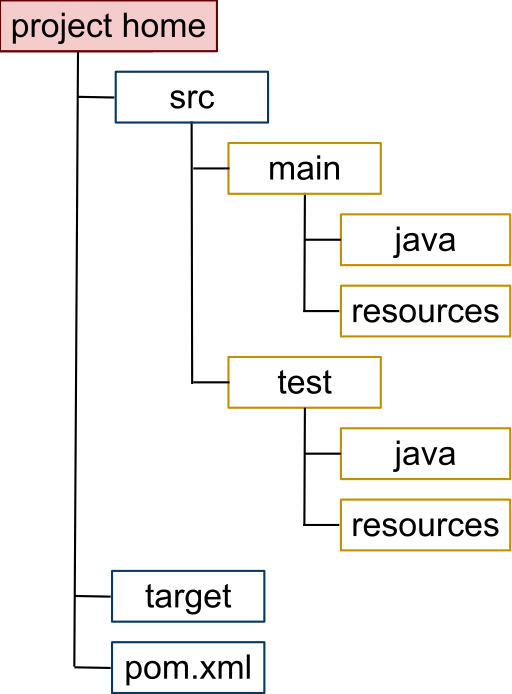
\includegraphics[scale=0.3]{figures/1}
\end{center}
\begin{compactitem}
\item project home	- Contains the pom.xml and all subdirectories.
\item src/main/java - Contains the Java source code for the project.
\item src/main/resources - Contains the deliverable resources for the project, such as property files.
\item src/test/java - Contains the testing source code (JUnit test cases, for example) for the project.
\item src/test/resources - Contains resources necessary for testing.
\end{compactitem}

%pom
A Project Object Model (POM) file contains at least the project's name
and its owner/organization name. For example here is an example of a
minimalistic POM file:


\begin{lstlisting}
<project>
  <modelVersion>4.0.0</modelVersion>
  <groupId>com.mycompany.app</groupId>
  <artifactId>my-app</artifactId>
  <version>1.0-SNAPSHOT</version>
</project>
\end{lstlisting}

As you can see  the POM file has XML structure and needs to have al
least the following elements:

\begin{compactitem}

\item project -  This is the top-level element in all Maven pom.xml files.

\item modelVersion -  This element indicates what version of the object
  model this POM is using. The version of the model itself changes
  very infrequently but it is mandatory in order to ensure stability
  of use if and when the Maven developers deem it necessary to change
  the model. It's default value is 4.0.0. 

\item groupId - This element indicates the unique identifier of the
  organization or group that created the project. The groupId is one
  of the key identifiers of a project and is typically based on the
  fully qualified domain name of your organization.
  This element must be specified and does not have a default value.

\item artifactId -  This element indicates the unique name of the
  primary artifact being generated by this project. The primary
  artifact for a project is typically a JAR file. A typical artifact
  produced by Maven would have the form artifactId-version.extension
  (for example, myapp-1.0.jar).
  This element must be specified and does not have a default value.

\item version - This element indicates the version of the artifact
  generated by the project. Maven goes a long way to help you with
  version management and the default version is 1.0-SNAPSHOT.

\end{compactitem}

Now let's really create a very simple maven project by invoking the
following command:

\begin{lstlisting}
$ mvn -B archetype:generate   -DarchetypeGroupId=org.apache.maven.archetypes   -DgroupId=com.mycompany.app   -DartifactId=my-app
\end{lstlisting}

The  important parameters of the command are groupID "com.mycompany.app" and
artifactID "my-app", archetypes are going to be discussed later. After
choosing an appropriate folder and running the above command in the
terminal maven will create the following folder structure and files: 

\begin{lstlisting}
$ tree
-- my-app
    |-- pom.xml
    |-- src
        |-- main
        |   -- java
        |       -- com
        |           -- mycompany
        |               -- app
        |                   -- App.java
        |-- test
            -- java
                -- com
                    -- mycompany
                        -- app
                            -- AppTest.java
\end{lstlisting}

As you can see, the project created has a POM file, a
folders for your application's sources and folders for your
test sources. This is the standard layout for Maven projects (the
application sources reside in src/main/java and test
sources reside in src/test/java.
In addition maven created a folder structure in both folders
reflecting the groupID you specified. It also included an App class
with a main method that prints "Hello world" in application sources
and an AppTest class hosting trivial JUnit tests for the App
class. Now let's inspect the POM file:

\begin{lstlisting}
$ cd my-app
$ cat pom.xml
<project xmlns="http://maven.apache.org/POM/4.0.0" xmlns:xsi="http://www.w3.org/2001/XMLSchema-instance"
  xsi:schemaLocation="http://maven.apache.org/POM/4.0.0 http://maven.apache.org/maven-v4_0_0.xsd">
  <modelVersion>4.0.0</modelVersion>
  <groupId>com.mycompany.app</groupId>
  <artifactId>my-app</artifactId>
  <packaging>jar</packaging>
  <version>1.0-SNAPSHOT</version>
  <name>my-app</name>
  <url>http://maven.apache.org</url>
  <dependencies>
    <dependency>
      <groupId>junit</groupId>
      <artifactId>junit</artifactId>
      <version>3.8.1</version>
      <scope>test</scope>
    </dependency>
  </dependencies>
</project>
\end{lstlisting}

This is a slightly more verbose POM file than the previous one and it
displays some addition POM elements, so let's walk through each of them:

\begin{compactitem}
\item packaging - This element indicates the package type to be
  created when building the project. Note that, this specifies both
  the artifact type produced (JAR, WAR, EAR, etc.) and a
  specific default lifecycle to use as part of the build process.
  The default value for the packaging element is JAR.

\item name - This element indicates the display name used for the
  project. This is often used in Maven's generated documentation. 

\item url - This element indicates where the project's site can be
  found. This is often used in Maven's generated documentation.

\item dependencies - This element describes all the external libraries
  used by the project. We will explain the dependency management later
  in more details.
\end{compactitem}

Usually a POM file is considerably more complex: defining multiple
dependencies and customizing plugin behavior. The first few
elements—groupId, artifactId, packaging, version—are what is known as
the Maven coordinates which uniquely identify a project. name and url
are descriptive elements of the POM providing a human readable name
and associating the project with a web site.

Maven always executes against an effective POM, a combination of
settings from this project’s pom.xml, all parent POMs, a super-POM
defined within Maven, user-defined settings, and active profiles. All
projects ultimately extend the super-POM, which defines a set of
sensible default configuration settings. While your project might have
a relatively minimal pom.xml, the contents of your project’s POM are
interpolated with the contents of all parent POMs, user settings, and
any active profiles. To see this complete and "effective" POM, run the
following command in the simple project’s base directory.
\begin{lstlisting}
$ mvn help:effective-pom
\end{lstlisting}

% archetype
Lastly, while creating the example project above we omitted some
details. We have used a particular plugin called Maven Archetype
plugin.
An archetype is a template for a Maven project which is used by the
Maven Archetype plugin to create new projects. Archetypes are useful
present end-users with a set of baseline projects that can be
used as a foundation for new applications. Archetypes can also be
useful within an organization that wants to encourage standards across
a series of similar and related projects. Anyone can create and publish
his/her own archetype that can be used by all other maven users.
Particularly, in the previous example we have used archetype called
maven-archetype-simple and for the lab project we suggest you to use
maven-archetype-quickstart archetype.
To create a project with a particular archetype you have to specify
the archetype's groupID and artifactID, for instance:

\begin{lstlisting}
$ mvn archetype:generate \
-DgroupId=com.mycompany.app \
-DartifactId=my-app \
-DarchetypeGroupId=org.apache.maven.archetypes \
-DarchetypeArtifactId=maven-archetype-quickstart \
-DinteractiveMode=false
\end{lstlisting}

\subsection{Project lifecycle}

To obtain an executable version of the application, the project must be
compiled, built and exported (as a .jar file, usually) with a
correctly configured classpath to all the classes of the
external libraries used in the project (i.e., dependencies) as well 
as the entry point class (i.e., the Main class). It is a
good practice to also test the application before using it.

Doing this manually every time would be cumbersome, thus in this
lab we will use Maven to automatize the build process.
Maven follows a build lifecycle when building the project. Build
lifecycle is a list of phases (also called maven goals) that must be
executed sequentially to build the project.

\begin{compactitem}
\item validate - validate if the POM file and project are correct and
  all necessary information is available

\item compile - compile the source code of the project

\item test - test the compiled source code using a suitable unit
  testing framework. These tests should not require the code be
  packaged or deployed

\item package - take the compiled code and package it in its
  distributable format

\item integration-test - process and deploy the package if necessary
  into an environment where integration tests can be run

\item verify - run any checks to verify the package is valid and meets
  quality criteria
 
\item install - install the package into the local repository, for use
  as a dependency in other projects locally 

\item deploy - done in an integration or release environment, copies
  the final package to the remote repository for sharing with other
  developers and projects

\end{compactitem}

When invoking a maven build you may specify any of the phases as a
goal of the build. Maven would then execute sequentially all phases
before the goal and the goal phase itself. For example, if you specify
\texttt{package} as a goal, phases \texttt{validate},
\texttt{compile}, \texttt{test} and \texttt{package} are going to be
executed.

Let's test this by packaging the application:

\begin{lstlisting}
$ mvn package
\end{lstlisting}

You’ve just created, compiled, tested and packaged the
simplest possible Maven project. To prove to yourself that this
program works, run it from the command line.

\begin{lstlisting}
$ java -cp target/my-app-1.0-SNAPSHOT.jar com.mycompany.app.App
Hello World!
\end{lstlisting}

An alternative (and easier) way to run a java project is using the
exec plugin of maven:

\begin{lstlisting}
$ mvn exec:java -Dexec.mainClass="com.mycompany.app.App"
\end{lstlisting}

The main difference between the two commands is that the exec plugin
would correctly specify the classpath of any runtime dependency, while
in the other case you would need to do this manually.

As you can see maven has created a jar of your application and placed
it in the target/ folder. In fact here is how the folder structure
looks like now:

\begin{lstlisting}
$ tree -L 2 .
|-- pom.xml
|-- src
|   |-- main
|   |-- test
|-- target
    |-- classes
    |-- maven-archiver
    |-- maven-status
    |-- my-app-1.0-SNAPSHOT.jar
    |-- surefire-reports
    |-- test-classes
\end{lstlisting}

If you perform the clean process, maven would delete all automatically
generated files:

\begin{lstlisting}
$ mvn clean
\end{lstlisting}

You can also customize individual phases of the build process. This is
implemented using plugins specified in the pom.xml file. Plugins are
other maven artifacts (i.e., they have their own groupID and
artifactID) that provide goals to Maven. Furthermore, a plugin may
have one or more goals wherein each goal represents a capability of
that plugin. For example, the Compiler plugin has two goals: compile
and testCompile. The former compiles the source code of your main
code, while the latter compiles the source code of your test code. 
Here is how you can modify the lifecycle of your project by
customizing the compile phase to use Java version 1.8:

\begin{lstlisting}
<project xmlns="http://maven.apache.org/POM/4.0.0" xmlns:xsi="http://www.w3.org/2001/XMLSchema-instance"
  xsi:schemaLocation="http://maven.apache.org/POM/4.0.0 http://maven.apache.org/maven-v4_0_0.xsd">
  <modelVersion>4.0.0</modelVersion>
  <groupId>com.mycompany.app</groupId>
  <artifactId>my-app</artifactId>
  <packaging>jar</packaging>
  <version>1.0-SNAPSHOT</version>
  <name>my-app</name>
  <url>http://maven.apache.org</url>
  <dependencies>
    <dependency>
      <groupId>junit</groupId>
      <artifactId>junit</artifactId>
      <version>3.8.1</version>
      <scope>test</scope>
    </dependency>
  </dependencies>
  <build>
    <plugins>
      <plugin>
        <groupId>org.apache.maven.plugins</groupId>
        <artifactId>maven-compiler-plugin</artifactId>
        <version>3.5.1</version>
        <configuration>
          <source>1.8</source>
          <target>1.8</target>
        </configuration>
      </plugin>
    </plugins>
  </build>
</project>
\end{lstlisting}



\subsection{Maven plugins}

We have just seen how using a particular maven plugin we can modify
the lifecycle of our project. However, plugins in maven have a much
more general use. 
The core functionality of Maven is very simple, it doesn’t know how to
do much beyond parsing a few XML documents and keeping track of a
lifecycle and a few plugins. In fact, Maven has been designed to
delegate most responsibility to a set of Maven Plugins which can
affect the Maven Lifecycle and offer access to goals. Most of the
action in Maven happens in plugin goals which take care of things like
compiling source, packaging bytecode, publishing sites, and any other
task which need to happen in a build. The Maven you download from
Apache doesn’t know much about packaging a WAR file or running JUnit
tests; most of the intelligence of Maven is implemented in the plugins
and the plugins are retrieved from the Maven Repository when they are
needed.

To execute a single Maven plugin goal, we used the syntax for instance
\begin{lstlisting}
 mvn archetype:generate
\end{lstlisting}
where archetype is the identifier of a plugin and
generate is the identifier of a goal.

\begin{center}
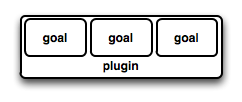
\includegraphics[scale=0.7]{figures/5}
\end{center}

A Maven Plugin is a collection of one or more goals. Examples of Maven
plugins can be simple core plugins like the Jar plugin, which contains
goals for creating JAR files, Compiler plugin, which contains goals
for compiling source code and unit tests, or the Surefire plugin,
which contains goals for executing unit tests and generating
reports.

\subsection{Dependency Management}

One of the central features of Maven is dependency management. If you
are developing a project that uses external libraries you do not need to
provide them together with your project. It is enough to specify the
dependency in the pom.xml file and during the build Maven will
automatically download the dependency and in turn, all the
dependencies that the dependency itself needs (called transitive
dependencies).

There are two types of repositories where maven searches for
dependencies: local and remote. Maven automatically creates a local
repository on your machine (usually on the .m2 folder) that contains
the cache of your downloaded dependencies, as well as the
builds of projects that you manage with maven. You can ``publish''
your project's artifact (a jar file, for instance) in you local maven
repository by invoking the install goal:

\begin{lstlisting}
$ mvn install
\end{lstlisting}

Now, for our example project with a groupId "com.mycompany.app", an
artifactId  "my-app", and a version "1.0-SNAPSHOT", the
install:install goal is going to copy the JAR file from
target folder to 
.m2/repository/com/mycompany/app/my-app/1.0-SNAPSHOT folder.
GroupID, artifactID and version are the so called maven project
coordinates. They are assumed to uniquely identify a project managed
with maven and can be used to look up any artifact published using
maven. You can now see from the example above maven coordinates can be
utilized to fetch the artifacts.

Maven also provides a remote ``Central Repository''  that is used by
default to search for dependencies, but other repositories can be
specified and used. You can browse available libraries at
\url{http://repo1.maven.org/maven2/}.

Again, you will see that the standard for a Maven repository is to store
an artifact in the following directory relative to the root of the
repository: 
\begin{lstlisting}
/<groupId>/<artifactId>/<version>/<artifactId>-<version>.<packaging>
\end{lstlisting}

Often you will be writing a project which depends on libraries that
are neither free nor publicly distributed. In this case you will need
to either setup a custom repository inside your organization's network
or download and install the dependencies manually.

\section{Maven Plugin for Eclipse (m2e)}

Maven Integration for Eclipse, named `m2e', provides the following features:
\begin{compactitem}
\item Launching Maven builds from within Eclipse
\item Dependency management for Eclipse build path based on Maven's pom.xml
\item Resolving Maven dependencies from the Eclipse workspace without installing to local Maven repository
\item Automatic downloading of the required dependencies from the remote Maven repositories
\item Wizards for creating new Maven projects, pom.xml and to enable Maven support on plain Java project
\item Quick search for dependencies in Maven remote repositories
\item Quick fixes in the Java editor for looking up required dependencies/jars by the class or package name
\end{compactitem}

What you need to understand is that the m2e plugin is only a
front-end graphical interface for maven. You can still use all the
maven features via command line, even if they are not supported by the
plugin. However, the typical use of maven for this course would not go
beyond the capabilities of the m2e plugin. 

\fi 

\subsection{Install Maven for Eclipse}

Maven is a standalone build tool that does not require you to use any
particular IDE. It is advisable for you to understand how Maven works
using the command line version since any particular Maven integration
with IDE will end up calling the exact same methods of the command
line version only wrapped in a (questionably) nice graphical interface.

One such interface is offered by the Eclipse plugin for Mavan
integration called m2e.

Eclipse 4.5.2 comes with installation of m2e, so the installation is
not needed. If you are using an older version of Eclipse (which is not
recommended) you can install latest m2e release by using the following
update site from within Eclipse: 

\url{http://download.eclipse.org/technology/m2e/releases/}

Perform following steps:
\begin{compactitem}
\item To to Help > Install New Software
\item Copy the above URL into the topmost textbox
\item Click on add and give it a name
\item After clicking OK, the list below should contain ''Maven Integration for Eclipse``
\item Check it
\item Click Next, Next, Accept, Finish
\end{compactitem}

An important caveat you need to be aware is that m2e plugin comes with
its own maven installation. Therefore, it is likely that building your
project via command line and via Eclipse might use different versions
of maven.

\ifinstall 
\else
\subsection{Create a Maven project in Eclipse}

This process is equivalent to the command line version of running:
\begin{lstlisting}
$ mvn archetype:generate 
\end{lstlisting}


The archetype generation need:
\begin{compactitem}
\item \textbf{Archetype}: kind of project we want to create
\item \textbf{Group ID}: Explanationar Id when my project includes multiple artifacts
\item \textbf{Artifact ID}: Identifier of the project
\item \textbf{Version}: 1.0 we are developing at the end we can release
\item \textbf{Package}: output of project web application (WAR) Enterprise application (EAR) Simple Java application (Jar)
\end{compactitem}

Archetype defines:
\begin{compactitem}
\item Folder structure
\item pom.xml
\end{compactitem}

To create a maven project:
\begin{compactitem}
\item Click File $>$ New $>$ Project ...
\item Choose Maven project
\item Click Next and choose \texttt{maven-archetype-quickstart} as
  shown in the figure:
\begin{center}
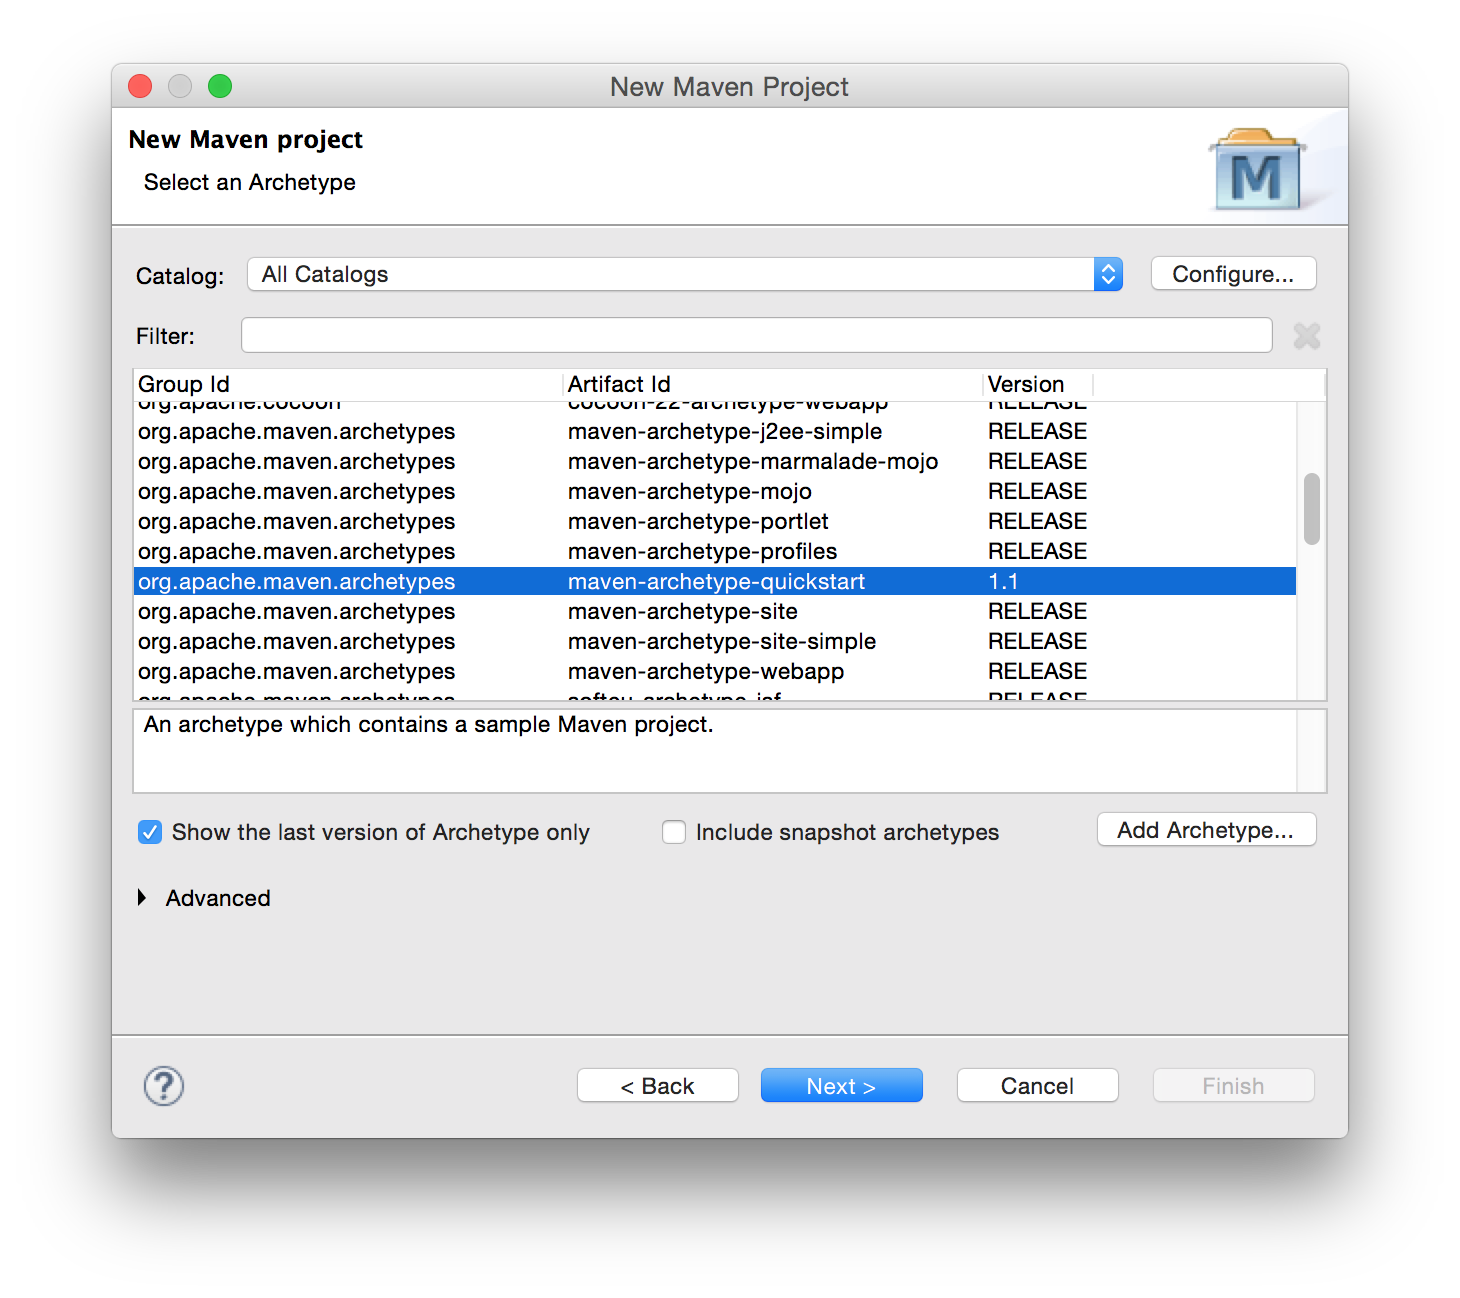
\includegraphics[scale=0.5]{figures/2}
\end{center}
\item Click Next. Set group ID to it.polimi.ingsw and artifact ID
  to 
  \prof*number* were *number* is the number of your group. You will
  be informed about your number by the lab responsibles. Figures show
  the example for project \prof01.
\begin{center}
\ifghezzi
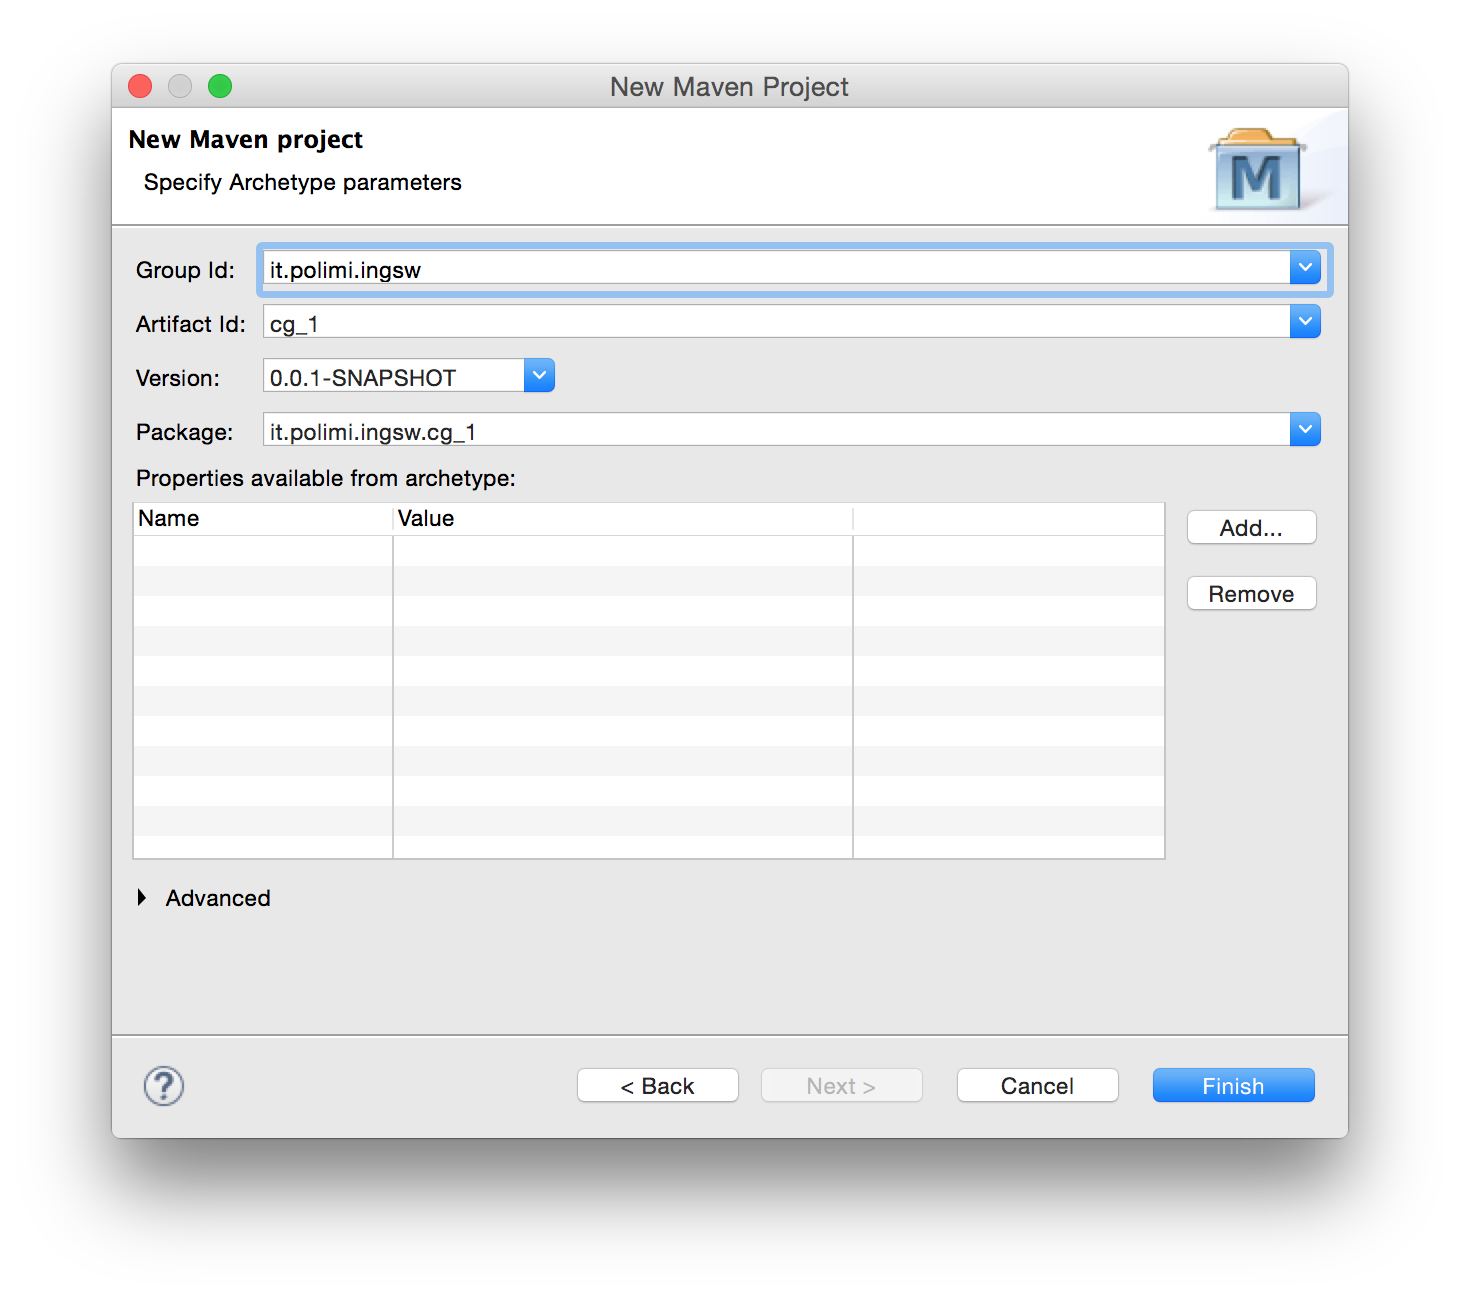
\includegraphics[scale=0.5]{figures/3}
\else
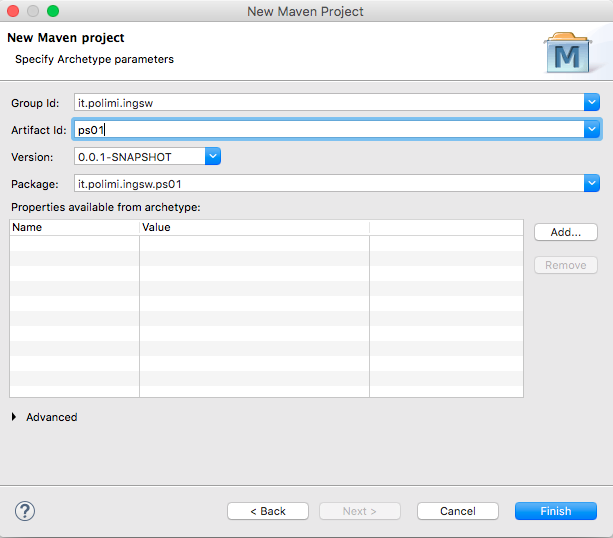
\includegraphics[scale=0.5]{figures/3ps}
\fi
\end{center}
\item Click finish and wait for the Maven to create the project. You
  should see the following structure of the project 
\begin{center}
\ifghezzi
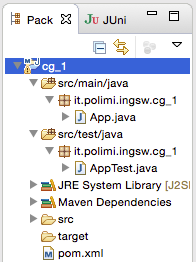
\includegraphics[scale=0.5]{figures/4}
\else
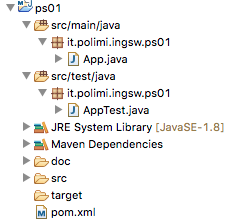
\includegraphics[scale=0.5]{figures/4ps}
\fi
\end{center}
\item Open pom.xml file (shown in the Package explorer on the left),
  choose the pom.xml tab in the lower part of the window and change it
  to match the pom.xml file shown below. Keep in mind to replace *professor\_code* with \prof{}  and   *number* with your appropriate number.
\end{compactitem}

\subsection{Create a Maven project in Eclipse}

\section{Pom.xml file for the lab}

\begin{lstlisting}
<project xmlns="http://maven.apache.org/POM/4.0.0" xmlns:xsi="http://www.w3.org/2001/XMLSchema-instance" xsi:schemaLocation="http://maven.apache.org/POM/4.0.0 http://maven.apache.org/xsd/maven-4.0.0.xsd">
  <modelVersion>4.0.0</modelVersion>
  <groupId>it.polimi.ingsw</groupId> 
  <artifactId>*professor_code**number*</artifactId> 
  <version>0.0.1-SNAPSHOT</version>
  <name>*professor_code**number*</name>
  <properties>
     <project.build.sourceEncoding>UTF-8</project.build.sourceEncoding>
     <sonar.language>java</sonar.language>
     <sonar.host.url> http://localhost:9000/ </sonar.host.url>
  </properties>
  <description>Prova Finale Ingegneria del software</description>
  <dependencies>
    <dependency>
      <groupId>junit</groupId>
      <artifactId>junit</artifactId>
      <version>4.12</version>
      <scope>test</scope>
    </dependency>
  </dependencies>
  <build>
    <plugins>
      <plugin>
        <groupId>org.apache.maven.plugins</groupId>
        <artifactId>maven-compiler-plugin</artifactId>
        <version>3.5.1</version>
        <configuration>
          <source>1.8</source>
          <target>1.8</target>
        </configuration>
      </plugin>
      <plugin>
	<groupId>org.jacoco</groupId>
	<artifactId>jacoco-maven-plugin</artifactId>
	<version>0.7.6.201602180812</version>
	<configuration>
	  <destFile>target/jacoco.exec</destFile>
	  <dataFile>target/jacoco.exec</dataFile>
	</configuration>
	<executions>
	  <execution>
	    <id>jacoco-initialize</id>
	    <goals>
	      <goal>prepare-agent</goal>
	    </goals>
	  </execution>
	  <execution>
	    <id>jacoco-site</id>
	    <phase>package</phase>
	    <goals>
	      <goal>report</goal>
	    </goals>
	  </execution>
	</executions>
      </plugin>
    </plugins>
  </build>
</project>
\end{lstlisting}

\fi

\end{document}




